%\section{Using Javascript}

As you become experienced with coding in ImageJ macros, you might start to find
out that for whatever you want to do with ImageJ, 
corresponding macro function does not exist in the Build-in Macro Functions page
\footnote{ see \url{http://rsb.info.nih.gov/ij/developer/macro/functions.html}}. 
One way to supplement the missing function is to create your own user function. 
Another way is to find a function directly from ImageJ Java code and use that function in macro. 
Javascript is a convenient way to access ImageJ API (Application Programming Interface), 
and since Javascript could be called from within ImageJ macro, you could use ImageJ API in your macro code. 
This is done by the macro function shown below:
\begin{shaded}
\begin{indentCom}
\item \textbf{eval("script", javascript)}\\
Evaluates the JavaScript code contained in the string javascript.\\
\end{indentCom}
\end{shaded}

This would be the simplest way to use Javascript if you are already
comfortable with ImageJ macro language. 

\textbf{But there is more to it}. You could also run Javascript as it is in
ImageJ and Fiji. Syntax of Javascript is not same as ImageJ macro, 
but if you are used to write ImageJ macro, it should not be too difficult to learn Javascript.  
 
\dots then how could we code Javascript? 

In this section, we learn basic know-how of 
Javascript with ImageJ 
\footnote{ If you want to learn in more detail, 
you could also visit \url{http://pacific.mpi-cbg.de/wiki/index.php/Javascript_Scripting} 
for learning more about Javascript.}. Experience with 
Java programming is largely helpful but if not, there is also some way around
to learn quickly. 

When we are programming ImageJ macro, we often refer to the
web site listing ImageJ macro language functions to look for a macro function. 
In similar way, we access so called API (Application Programming Interface) 
for coding with Javascript. ImageJ API is in the following page:

\url{http://rsb.info.nih.gov/ij/developer/api/index.html}

At this moment, you might be puzzled with these pages, 
but don't worry. Major aim of this section is to learn how to use this resource 
to code your Javascript. 

OK, let's start. 

\subsection{A trial with Javascript}
%
Let us first try using Javascript (JS). 

From menu, do \ijmenu{[Plugins > Scripting > Javascript Interpreter]}. 
You will then see a new interface that looks like Fig \ref{fig:JSinterpreter}. 
This interface provides Javascripting in an interactive mode and is useful for 
a quick testing of codes. There is a input field at the bottom, where you could type in JS code. 
Then by pressing return key, the code is executed.  

\begin{figure}[htbp]
\begin{center}
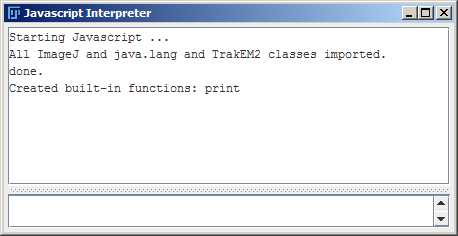
\includegraphics[width=100mm]{fig2/JSinterpreterStasrtUp.png}
\caption{Javascript interpreter on start up.}
\label{fig:JSinterpreter}
\end{center}
\end{figure} 

Type the following command and execute by return key. 
\begin{lstlisting}[numbers=none]
IJ.log("Hello JS")
\end{lstlisting}
This JS command will print "Hello JS" in the Log window of ImageJ.  

Same command could be written in the Script editor. To start up the editor, 
do \ijmenu{[File > New > Script]} (then select \ijmenu{[Language > Javascript]}). 
\begin{lstlisting}[numbers=none]
IJ.log("Hello JS");
\end{lstlisting}
This should do the same thing, but be careful! Do not forget adding semicolon
(;) at the end of the line. In case you write your code in Script Editor, you need
to explicitly mark the end of line, just like you do when you write a macro.

To run the code, \ijmenu{[Run > Run]} will execute the command (you could also
use ctrl-r or cmd-r). 

What this JS code does is the same as the Macro code below. 
\begin{lstlisting}[numbers=none]
print();
\end{lstlisting}

In the following, you could use either Javascript interpreter 
or Script editor. Just choose the one you like. If code become multiple lines, 
I recommend you to use the Script Editor\ldots and in this case, this is a
redundant warning, place a semi-colon ``;'' at the end of each line.

Now, we could try some commands that is not present in 
ImageJ macro.
 
For example, what would you do if you want to convert angle in degrees to radian? 
In macro, you could do calculation by first dividing the value by 360, 
then multiply by $2\pi$. But a function actually is already there in Java, 
so you could simply use that as well. 
\begin{lstlisting}[numbers=none]
IJ.log(java.lang.Math.toDegrees(3.1415)) 
\end{lstlisting}
Running this line should print a number close to 180. You could also do the
other way around:
 \begin{lstlisting}[numbers=none]
IJ.log(java.lang.Math.toRadians(180)) 
\end{lstlisting}
should print out 3.1415\dots.

Next, we try to retrieve a column of data from table in Results window. 
In macro, you could do this by \ilcom{getResult} function, 
with which by specifying the column label and row number you could retrieve 
a value in that cell. 

But what should we do if we want to retrieve all data in a row at once, 
not a single value in a specific column at specific row? 
If you want to do this in macro, we could write a user defined function that loops 
for all the columns and get data one-by-one. 

With Javascript, this could be done in just a single step, one command. 

\begin{indentexercise}{1}

\textbf{Preparation of Results table}

Open image by \ijmenu{[File > Open Sample > blobs (25k)]}. 

Check measurement parameters by 

\ijmenu{[Analyze > Set Measurements\dots]}

that some measurement parameters are checked. Be sure that "Limit to Threshold" is checked. 

Then Threshold the blob image by 

\ijmenu{[Image > Adjust > Threshold]}. 

Since the background of this image is bright, Dark Background' should be unchecked. 
If you see the thresholded image like fig. \ref{fig:ThresBlob},  do 

\ijmenu{[Analyze > Analyze Particles\dots]}. 

%figure
\begin{figure}[htbp]
\begin{center}
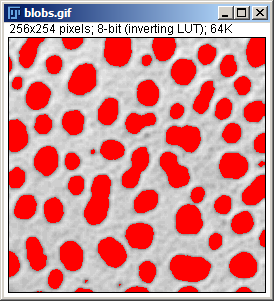
\includegraphics[height=50mm]{fig2/ThrehsoldedBlob.png}
\caption{Thresholded image of "blob"}
\label{fig:ThresBlob}
\end{center}
\end{figure} 

In the Analyze Particles dialog, just be sure that \textbf{Display Results} is checked. 
Then click OK button. When the analysis is done, you will see  64 or so particles detected 
and listed in the Results window. 

\textbf{Testing Javascript Code}

We now use the following command to extract data from single Row. In Javascript
interpreter, type the following command .

\begin{lstlisting}[numbers=none]
IJ.log(ResultsTable.getResultsTable().getRowAsString(10));
\end{lstlisting}

If you execute this, you will see that all data that is in row 11 in Results table is 
now printed in the log window. 

\dots that's the end of this exercise but don't close the Results window yet.   
\end{indentexercise}

Above is a single line pure JS code. 
We can use this code within macro by using \textbf{eval} function mentioned already. 
Here is an exercise to test the function \textbf{eval}. 

\begin{indentexercise}{2}
Test running the following code, and check that any row in the table could be extracted 
and printed in Log window. 
\begin{lstlisting}
rownum = getNumber("Row?", 0);
jscom = "IJ.log(ResultsTable.getResultsTable().getRowAsString("+rownum+"));";
eval("script", jscom);
\end{lstlisting}
\end{indentexercise}

In the second line, JS code is constructed as a single string \ilcom{jscom} 
using the variable \ilcom{rownum} from line 1. Line 3 executes this JS code using \textbf{eval}. 

So far, I have not yet explained where these commands came from. 
I will give more detailed explanation in later sections.  

\begin{indentexercise}{2}
This exercise is optional:

Try the following Javascript commands using \textbf{eval}, from within an ImageJ
macro.

\dots lists all ImageIDs. There should be at least one image opened. 
\begin{lstlisting}[numbers=none]
a = WindowManager.getIDList();
for(i in a) IJ.log(a[i]);
\end{lstlisting}

\dots zooms current image centered at top-left corner.
\begin{lstlisting}[numbers=none]
IJ.getImage().getCanvas().zoomIn(0, 0);
\end{lstlisting}

\dots print souts statistics of current image in log window.
\begin{lstlisting}[numbers=none]
eval("script", "IJ.log(IJ.getImage().getStatistics().toString());");
\end{lstlisting}

\dots print outs used memory in log window.
\begin{lstlisting}[numbers=none]
eval("script", "print(IJ.currentMemory())");
\end{lstlisting}

\dots moves current image window to top-left corner of the monitor with offset of 10 by to, 
and resizes the window. 
\begin{lstlisting}[numbers=none]
eval("script", "IJ.log(IJ.getImage().getWindow().setLocationAndSize(10, 10, 100, 100))");
\end{lstlisting}
\end{indentexercise}

In all the example codes, we placed Javascript commands in the second argument 
for the function \textit{eval}. 
You could also write a full path to a Javascript file. Here is the syntax. 
\begin{shaded}
\begin{indentCom}
\item \textbf{eval}('script', \textbf{File.openAsString}("<pathpath>/name.js")) ;
\end{indentCom}
\end{shaded}

\subsection{Using Macro Recorder and ImageJ API}
Javascript is a scripting language, so it has its own build-in functions. 
I will not explain about this since you could find many Javascript tutorials on the web. 
For example, following site is a place where I go and look for Javascript commands and usages:

\href{http://www.w3schools.com/jsref/default.asp}{Javascript Reference @ w3chools.com}

How do we find Javascript commands to interact and control ImageJ? 
The easiest way is to use the macro recorder. 
We have already learned and used macro recorder in previous chapters. 
We could used the same interface for recording JS codes. 
Recorded lines of JS codes could be copy \& pasted into Script Editor and can be directly executed. 

\begin{indentexercise}{1}
First, we should start the recorder. 
\ijmenu{[Plugins > Macros > Record\dots]}. 
Then in the recorder window at the top-left corner, 
choose Javascript as the code to be recorded (Fig. \ref{fig:MacroRecorderJS}). 

%figure
\begin{figure}[htbp]
\begin{center}
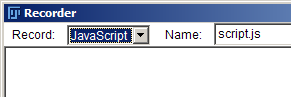
\includegraphics[width=70mm]{fig2/RecorderJS.png}
\caption{Setting Up Macro Recorder ready for Javascript}
\label{fig:MacroRecorderJS}
\end{center}
\end{figure}

Then do the following sequence of commands.
\begin{itemize}
\item \ijmenu{[File > Open Sample > Blobs]}
\item Select rectangular ROI tool and set a ROI to select 
about 1/4th of the image (can be any place within the image. This is just a test.). 
\item \ijmenu{[File > Transform > Flip Horizontally]}
\item \ijmenu{[Process > Filters > Gaussian Blurr\dots]}
\end{itemize}
After all these operations, there should be JS codes printed in the Recorder window. 
Copy them all, and paste it to Script Editor (\ilcom{[File > New > Scripts]} and then paste, 
Fig. \ref{fig:ScriptEditorRecorded}) . 
After pasting, set language to JS by (\ilcom{[Language > Javascript]} from the menu bar of script editor.  

%figure
\begin{figure}[htbp]
\begin{center}
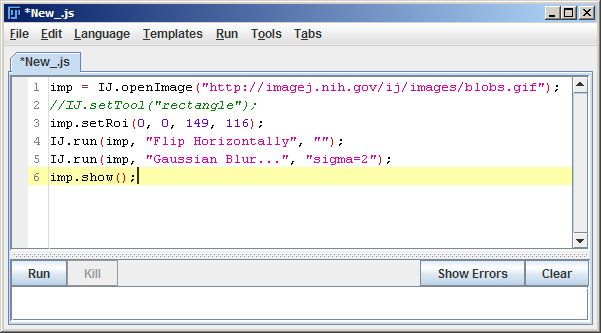
\includegraphics[height=50mm]{fig2/JSrecordedInScriptEditor.png}
\caption{Javascript by recorder commands.}
\label{fig:ScriptEditorRecorded}
\end{center}
\end{figure}

Then do \ilcom{[Run > Run]} from the menu of script editor, the script is executed. 
You should then see a new window of "blob" with some part of image processed. 
\end{indentexercise}
If you are successful in running the code, let's see the code. Here is how the code should look like. 

%\lstinputlisting[morekeywords={*}]{code/code29.js}
\lstinputlisting{code/code29.js}

We first examine line 3 and line 4, focusing on the method \ilcom{IJ.run}  
(in the follwoing, we use word "method" instead of "command", as this is more 
conventional way of calling it in Java). This method has three arguments for it.

\ilcom{IJ.run(argument1, argument2, argument3)}

 Just by looking at each of them you could realize that the second argument 
 is a descriptive explanation of what the method does. 
 This is because these strings are exactly the phrase of the menu item you see 
 when you choose that function from ImageJ menu. 

\ilcom{IJ.run} is a method that uses second argument as a keyword 
to search for all the ImageJ menu items to find which of them is the one 
that the method intends to invoke 
\footnote{In ImageJ macro, a function similar to \ilcom{IJ.run} 
method is \ilcom{run(arg1, arg2)}.}. 
Third argument of \ilcom{IJ.run} in line 3 is an empty string, 
but in line 4, the third argument is \ilcom{sigma=2}. 
This is a value that you normally input when you select Gaussian blur 
from the menu bar for the size of blurring kernel. 

Then what is the first argument in \ilcom{IJ.run}? 
In both line 3 and 4, we have a variable \textbf{\ilcom{imp}}. 
To see what this is, we go back to line 1. 
\textbf{\ilcom{imp}} appears for the first time in the code at line 1, 
and \textbf{\ilcom{imp}} is the returned value of a method \ilcom{IJ.openImage}. 
If we think back what we were actually doing for this first line when recording, 
we accessed an item in the menu tree \ijmenu{[File > Open Sample > blobs]}. 
By choosing this item from menu, ImageJ downloads blobs.gif file from NIH web site 
and then shows it on your desktop. 
Single method that does the download action is the method \ilcom{IJ.openImage}. 
Argument for this command is the URL of the image. 

To know the definition of the method \ilcom{IJ.openImage}, 
we look up a reference called 
\href{http://rsb.info.nih.gov/ij/developer/api/index.html}{ImageJ API}
\footnote{ ImageJ API: http://rsb.info.nih.gov/ij/developer/api/index.html}. 
In this web page, there is side bar in left side, with upper part 
for a list of "All Packages" 
(These packages are same as those listed in the table shown in the top page) 
and the bottom part for "All Classes".  

%figure
\begin{figure}[htbp]
\begin{center}
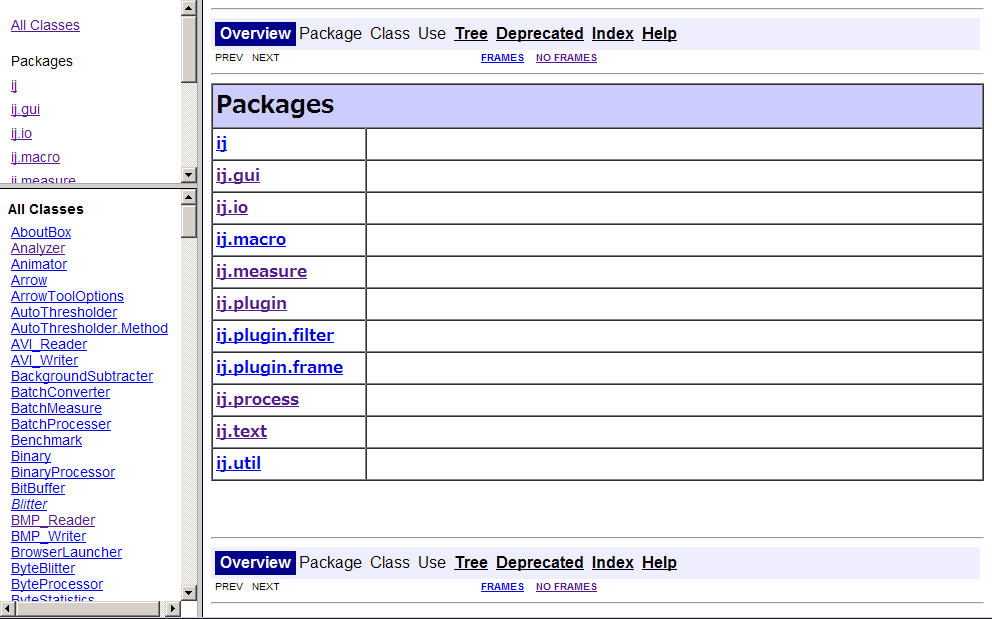
\includegraphics[height=75mm]{fig2/IJAPItop.png}
\caption{ImageJ API}
\label{fig:IJAPItoppage}
\end{center}
\end{figure}


Each package contains several classes. 
We currently do not know which package does 
\ilcom{IJ.openImage} belong to, so we look for it in the bottom part "All Classes". 
There, you will find "IJ"\footnote{ Unlike ImageJ macro, Java and Javascript are case sensitive}. 
Click the link, and in the right side of the page, a page titled "Class IJ" appears 
(Fig. \ref{fig:IJAPClassIJ}). 

%figure
\begin{figure}[htbp]
\begin{center}
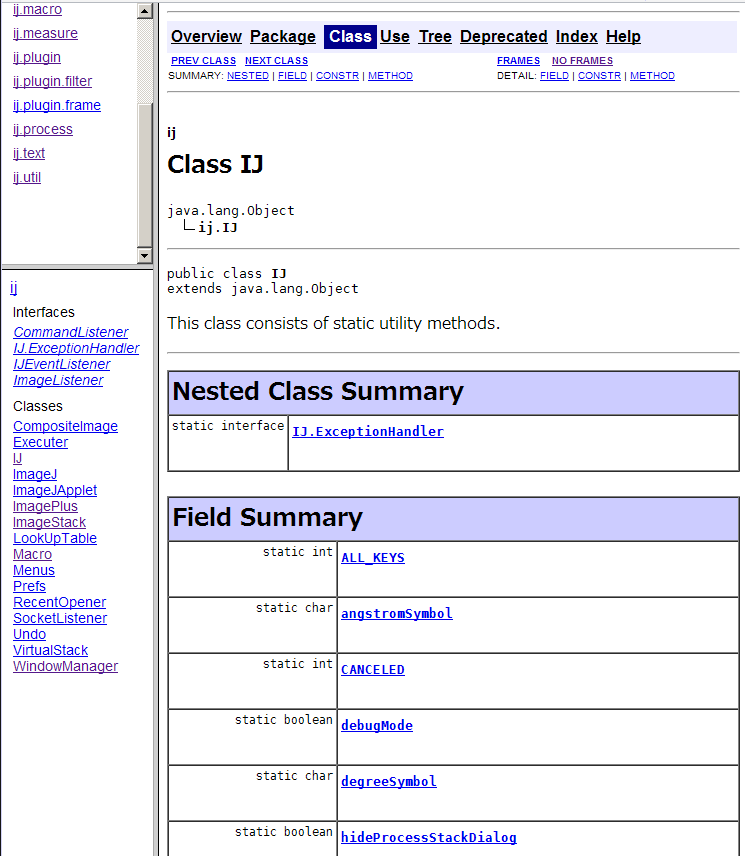
\includegraphics[width=75mm]{fig2/IJAPI_IJ.png}
\caption{ImageJ API Class IJ}
\label{fig:IJAPClassIJ}
\end{center}
\end{figure}

The page might look cryptic to you, if you scroll down the page, there is a table titled "Method Summary", listing all the methods that class IJ contains in alphabetical order. 
Within this list, you will find (Fig. \ref{fig:IJAPIIJopenImage})

\ilcom{openImage(java.lang.String path)} 


%figure
\begin{figure}[htbp]
\begin{center}
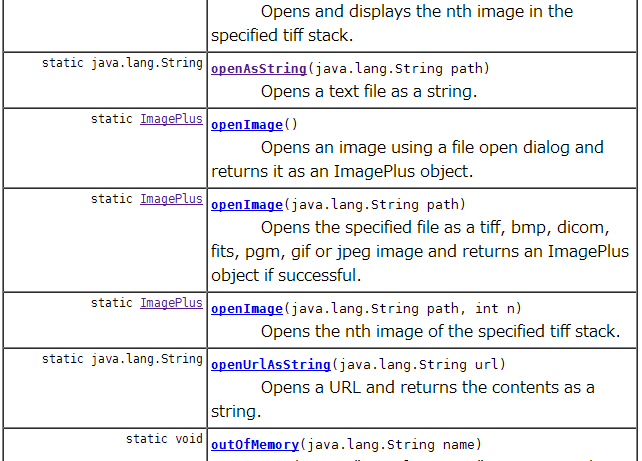
\includegraphics[height=75mm]{fig2/IJAPI_IJopenImage.png}
\caption{ImageJ API Class IJ, openImage method}
\label{fig:IJAPIIJopenImage}
\end{center}
\end{figure}

There are three \ilcom{openImage} methods, with difference in number and types of arguments. 
The first one is without any argument, the second one has only one argument, 
the third having two arguments. 
When openImage method is called, one of these three are called depending on the number 
and types of the argument in the call. 

\textbf{More Explanation:} So what are "Classes?" A class consists of two major components. 
One is Field and the other is Method. 
The former is like variable and the latter is similar to function in ImageJ macro 
(this is not a precise analogy, but for now let's think like that). 
Fields are values. Methods are actions. Class is a group of various field values and methods. 
By utilizing Class, we can have a single unit of assembled functions, 
which would be an advantage for letting an application to have high modularity. 
You could access (or use) fields and methods by appending them behind the name
of the class. For example. <class name>.<field name> or <class name>.<method name>(<arguments>) 
e.g. \ilcom{IJ.openImage(pathname)}.

 \textbf{A bit more on API page} At the top of the Class IJ page (Fig.\ref{fig:IJAPClassIJ}), 
 "ij" is written above the class name "Class IJ". 
 This is the name of package that is containing this class. 
 You could see all classes within the package ij (note: case sensitive), 
 click "ij" in the left top panel listing "all packages".  
 You then will see all the classes within the package ij, 
 such as compositeImage, Executor, IJ, ImageJ\dots and so on. 
 Package is used to organize classes in hierarchical tree. 
 For example, there are packages ij.plugin, ij.plugin.filter and ij.plugin.frame. 
 Likewise, package is a tree-like structure (remember how folders are organized in your laptop) 
 that organizes many classes in a structure. In Java, such tree-like structure
 is organized separated by dots (``.''). For example, see
 \href{http://rsb.info.nih.gov/ij/developer/api/ij/plugin/filter/package-summary.html}{Package
 ij.plugin.filter}. The package filter is under the plugin package, that is
 under the ij package. 
  
Go back to the API description, in the left side of the table column where 

\ilcom{openImage(java.lang.String path) } 

is listed (Fig. \ref{fig:IJAPIIJopenImage}), there is a phrase 

\ilcom{static ImagePlus} 

This tells you that if you invoke method \ilcom{openImage(java.lang.String path)} of class \ilcom{IJ}, 
a object called ImagePlus is returned (forget about the notion "static" for now). 
ImagePlus is another class, which you could also look up using the list of "All Classes".  

The class ImagePlus consists of image data and metadata fields, and methods to access these values. 
In \href{http://rsb.info.nih.gov/ij/developer/api/ij/ImagePlus.html}{ImagePlus API page}, 
you could see that many fields and methods are associated with this class. 
Note that many of field values are "protected". 

For example, \ilcom{nChannels} is one of the filed values of class ImagePlus 
but having a notion "protected" means that you cannot simply access from outside the class itself. 
Instead, there is a method named \ilcom{getNChannels()} for accessing the value 
from outside which by invoking it "Returns the number of channels" of ImagePlus object. 
\ilcom{getNChannels()} returns a value indicated as "int". 
This tells you that the type of returned object is "int", which means that returned value is a number, 
and specifically an integer, not a number with decimal points. Unlike ImageJ macro 
\textbf{object} with any type of class could be returned, not limited to number, string and array. 
This flexibility affords higher potential in modularity with Javascript compared to ImageJ macro 
and hence we call returned values as "object" not "variables". 

A draw back is that Javascript coding becomes a bit more complicated then macro
coding. One should always be careful about which class or type is returned, 
and one way to do so is to check ImageJ API every time you wonder what is the
returned value of certain method.

Let's go back to the code again. 
The method \ilcom{IJ.openImage} returns an \textbf{object "ImagePlus"}, 
so in line 1 of the recorded Javascript code, 
an instance of ImagePlus object (which actually is "blob.png" downloaded from the NIH website) 
is stored in the variable "imp". 
Then after line 1, \ilcom{imp} behaves as an ImagePlus object. 
\ilcom{imp} is repeatedly used from line 2 to 5. In line 2, an method of class ImagePlus is invoked 
in the form <class>.<method>(arguments). 
Since method name is \ilcom{setROI} we look for it in the 
\href{http://rsb.info.nih.gov/ij/developer/api/ij/ImagePlus.html}{ImaegJ API ImagePlus page}, 
and you will find the following description:

\begin{quote}
void | setRoi(int x, int y, int width, int height) \\
          Creates a rectangular selection.
\end{quote}

"void" means that this method does not return any value. 
There are four arguments and all of them are "int", integer. 
Description tells you that this methods creates an ROI in the image with position and size 
defined by arguments.  

In line 3 and 4, the first argument of \ilcom{run} method is \ilcom{imp}, 
telling the command \ilcom{IJ.run} to do the operation specified by the second argument on \ilcom{imp}. 

Note that in case of ImageJ macro, target image could only be specified by 
activating the window using \ilcom{selectImage(imageID)}. 
In Javascript, selection of image could be more explicit by the direct use of ImagePlus object.  

Down to line 4, blob image actually is not shown on the desktop. 
ImagePlus object of "blobs.tif" is in the memory, but still is not displayed. To
show it on the desktop, we do line 5.

\begin{quote}
\ilcom{imp.show();}
\end{quote}

\ilcom{show()} is a method of ImagePlus class to show the actual image of ImagePlus object. 

%In case of Macro, we could execute that as a single line. 
% So how about doing the same? 
% Create a new script tab by \ijmenu{[File > New]} 
% from the script editor menu. 
% Then copy line 4 and paste that single line in the new script.

\textbf{Grabbing Image}
What if you want to capture already opened Image as a ImagePlus object? 
This could be done by using a method in Class IJ called \ilcom{getImage()}. 
You could replace the first line in the code we just studied with \ilcom{IJ.getImage()} 
to grab currently active image rather than downloading and opening an image file. 

\begin{indentexercise}{1}
Modify code 29 so that this JS code grabs currently active image and do the same processing. 
\end{indentexercise}

\begin{indentexercise}{2}
We study the nature of ImagePlus object in this exercise. We start with a simple
code to open an image, then add more lines to see how ImagePlus instance
behaves. Type in the code below to start up. 

\lstinputlisting{code/code30_1.js}

As we have done already, this will show a blobs.gif image on your desktop. We
can have another window with blobs.gif by adding two more lines. 

\lstinputlisting{code/code30_2.js}

We now have two instances of ImagePlus object. These are independent. 
Whatever you do to imp, that does not affect imp2. We could do a small trick
that two windows could share the the same image, that the same image appearing
in two windows. Close two windows of blobs, and then modify the code as shown
below.

\lstinputlisting{code/code30_3.js}

Run this code, and you would see two windows with same image, which seemingly
are same as before. 

Take one image and try to select some region using a ROI tool,
and from Fiji menu do \textit{[Edit > delete]}. Then the selected region blacks
out or whites out. Click another blobs window. Then you would see that the
second window, which you did not process anything, also is processed. 

This is because both windows are sharing the same image, shown in two windows.
In other way of saying, there is a single instance of image with two ImagePlus
instances. In the modified code, an extra line is added in line 3, and line 4 is
changed. Line 3 is generating a pointer (ip) to the image that is contained in
the ImagePlus instance \textit{imp}. In the 4th line, a new instance of
ImagePlus is created using what we call ``constructor'' (see ImagePlus API for
a list of constructor), using the ip that is actually associated with the
preexisting ImagePlus \textit{imp}. Finally, the 5th line shows the second
window \textit{imp2}, the image content of which is shared with \textit{imp}. 
 
\end{indentexercise}

\textbf{Summary}
\begin{itemize}
\item Object should be either created (initialized, of "Constructed") or Grabbed. 
\begin{itemize}
\item \ilcom{IJ.openImage(path)} creates and image object from file.
\item \ilcom{IJ.getImage()} grabs already existing object. 
\end{itemize}
\item Object is constructed taking a class as template. A class has field values and methods. 
Hence, object has those values and classes. 
\begin{itemize}
\item Field values are in most cases accessed via methods.
\item Once an object is constructed, its public method could be used
\end{itemize}
\item Exception: So called "static" methods could be accessed any time. 
\begin{itemize}
\item Most of methods in Class IJ are static, so you do not need to construct
it.
\end{itemize}
\end{itemize}

\subsection{Example Codes}

In this section, I will just show Javascript example using ImageJ
API\footnote{Javascript cookbook is also available in the CMCI website for
various coding examples. Visit
\url{http://cmci.embl.de/documents/110822jsip_cooking/javascript_imagej_cookbook}}.

Curve Fitting example. 
\lstinputlisting{code/codeCurveFitting.js}


\subsection{Using none-ImageJ libraries in Fiji}

Besides access to ImageJ API, power of Javascript is in importing external packages 
written in Java to use their functions.

In Fiji, many java libraries (packages) are included besides ImageJ itself. 
You could see them listed in \href{http://fiji.sc/javadoc/}{Fiji API}. 
Here are some picks among them, which might be interesting to use for math and statistics 
in Javascript\footnote{ If you want to use these packages in ImageJ, 
you could download the package from its website and configure ImageJ 
to include that package on start up.}. In the next section, 
we will study several examples to know how to import these libraries in Javascript. 

\href{http://math.nist.gov/javanumerics/jama/}{Java Matrix Package (JAMA)}
\begin{shaded}
\begin{quote}
 JAMA is comprised of six Java classes: Matrix, CholeskyDecomposition, 
 LUDecomposition, QRDecomposition, SingularValueDecomposition and EigenvalueDecomposition.

The Matrix class provides the fundamental operations of numerical linear algebra. 
Various constructors create Matrices from two dimensional arrays of double precision 
floating point numbers.  Various gets and sets provide access to submatrices and matrix elements. 
The basic arithmetic operations include matrix addition and multiplication, 
matrix norms and selected element-by-element array operations.  
A convenient matrix print method is also included.

Five fundamental matrix decompositions, which consist of pairs or triples of matrices, 
permutation vectors, and the like, produce results in five decomposition classes.  
These decompositions are accessed by the Matrix class to compute solutions of simultaneous linear equations, 
determinants, inverses and other matrix functions.  The five decompositions are
\begin{itemize}
\item Cholesky Decomposition of symmetric, positive definite matrices
\item LU Decomposition (Gaussian elimination) of rectangular matrices
\item QR Decomposition of rectangular matrices
\item Eigenvalue Decomposition of both symmetric and nonsymmetric square matrices
\item Singular Value Decomposition of rectangular matrices
\end{itemize}
\end{quote}
\end{shaded}

\href{http://commons.apache.org/math/}{Apache Commons Math Package}
\begin{shaded}
\begin{quote}
Commons Math is divided into fourteen subpackages, based on functionality provided.
\begin{itemize}
\item org.apache.commons.math.stat - statistics, statistical tests
\item org.apache.commons.math.analysis - root finding, integration,
interpolation, polynomials
\item org.apache.commons.math.random - random numbers, strings and data generation
\item org.apache.commons.math.special - special functions (Gamma, Beta)
\item org.apache.commons.math.linear - matrices, solving linear systems
\item org.apache.commons.math.util - common math/stat functions extending java.lang.Math
\item org.apache.commons.math.complex - complex numbers
\item org.apache.commons.math.distribution - probability distributions
\item org.apache.commons.math.fraction - rational numbers
\item org.apache.commons.math.transform - transform methods (Fast Fourier)
\item org.apache.commons.math.geometry - 3D geometry (vectors and rotations)
\item org.apache.commons.math.optimization - function maximization or minimization
\item org.apache.commons.math.ode - Ordinary Differential Equations integration
\item org.apache.commons.math.genetics - Genetic Algorithms
\end{itemize}
\end{quote}
\end{shaded}

\href{http://xmlgraphics.apache.org/batik/}{Batic SVG Tool kit}
\begin{shaded}
\begin{quote}
Batik is a Java-based toolkit for applications or applets that want to use images 
in the Scalable Vector Graphics (SVG) format for various purposes, 
such as display, generation or manipulation.

The project's ambition is to give developers a set of core modules 
that can be used together or individually to support specific SVG solutions. 
Examples of modules are the SVG Parser, the SVG Generator and the SVG DOM. 
Another ambition for the Batik project is to make it highly extensible—for example, 
Batik allows the developer to handle custom SVG elements. 
Even though the goal of the project is to provide a set of core modules, one of the 
deliverables is a full fledged SVG browser implementation which validates the various modules 
and their inter-operability.
\end{quote}
\end{shaded}

\href{http://spaceroots.org/software/mantissa/index.html}
{Mantissa (Mathematical Algorithms for Numerical Tasks In Space System Applications)}
\begin{shaded}
\begin{quote}
Mantissa is a collection of various mathematical tools aimed towards for simulation. 
It is not a complete mathematical library like GSL, NAG or IMSL, but it contains various 
algorithms useful for dynamics simulation and 3D geometry computation.
\end{quote}
\end{shaded}

\href{http://www.cs.waikato.ac.nz/ml/weka/}{Weka}
\begin{shaded}
\begin{quote}
Weka is a collection of machine learning algorithms for data mining tasks. 
The algorithms can either be applied directly to a dataset or called from your own Java code. 
Weka contains tools for data pre-processing, classification, regression, 
clustering, association rules, and visualization. 
It is also well-suited for developing new machine learning schemes.
\end{quote}
\end{shaded}

Some other packages\dots

\begin{itemize}
\item \href{http://www.imagescience.org/meijering/software/}{ImageScience} - 
Implemented as plugins for filtering but valuable for use as a library. 
\item \href{http://www.f4.htw-berlin.de/~barthel/ImageJ/ImageJ3D/ImageJ3D.html}
{ImageJ3D - JRenderer3D} -3D renderer. 
\item kfschmidt.*  - Numerical analysis tools: Simplex, GLM analyzer, Matrix
calculations
\item math3D -Matrix calculation, 3D tools.  
\end{itemize}

\subsection{Example Use of Library}
Following will be some examples of using Apache Commons Math library. 
\subsubsection{Descriptive statistics}

\lstinputlisting{code/code32.js}

When you use a package, you should first import it. 
The first line is doing this by using a method \ilcom{importPackage}. 
One could also import a single class, using \ilcom{importClass} method. 
In line 4, a new object of Class DescriptiveStatistics is created. Line 5 and 6 stores data in this object, 
and calculates statistics in line 9, 10 and 11.

\subsubsection{Solving Linear System}
% http://commons.apache.org/math/userguide/linear.html
We could solve linear equation system below, in the form AX = B, by LU decomposition. 
\[
2x + 3y - 2z = 1
\]
\[
-x + 7y + 6x = -2
\]
\[
4x - 3y - 5z = 1         
\]

\lstinputlisting{code/code33.js}

\newpage
